% 导言区,进行全局设置
%\documentclass[oneside, 12pt, twocolumn]{ctexbook}%book, report, latter, 引入文档类
\documentclass[oneside, 12pt]{ctexbook}

%\usepackage{ctex}
%\usepackage[fleqn]{amsmath}
\usepackage{amsmath}
\usepackage{amssymb}
\usepackage{fancyhdr}
\usepackage{lastpage}
\usepackage{graphicx}
\usepackage{float}
\usepackage{enumerate} % when need define format to number by myself
\usepackage[colorlinks,linkcolor=black]{hyperref} % set super link
\usepackage{color} % set text color
\usepackage{subfigure} % set two picture on one line

\usepackage{geometry}
\geometry{a4paper,top=2.54cm,left=3.18cm,bottom=2.54cm,right=3.18cm,includehead,includefoot}

% \newcommand命令的定义,新的命令
\newcommand\degree{^\circ}
\title{\kaishu Support Vector Machine}
\author{Fish}
\date{\today}

\graphicspath{{figures/}} %图片在当前目录下的figures目录

% 内容与格式分离
% 设置标题的格式
\ctexset {
	section = {
		format+=\zihao {-4} \heiti \raggedright,
		%name = {,},
		%number = \chinese{section},
		beforeskip = 1.0ex plus 0.2ex minus .2ex,
		afterskip = 1.0ex plus 0.2ex minus .2ex,
		aftername = \hspace{0pt}
	},
	subsection = {
		format+=\zihao{5} \heiti \raggedright,
		% name={\thesubsection},
		name = {,},
		%number = \arabic{subsection},
		beforeskip = 1.0ex plus 0.2ex minus .2ex,
		afterskip = 1.0ex plus 0.2ex minus .2ex,
		aftername = \hspace{0pt}
	}
}


% 正文区(文稿区),有且只有一个document环境
% \begim{*环境名称}
%        内容
% \end{*环境名称}
\begin{document}
	\maketitle
	%\clearpage
	\cleardoublepage
	\thispagestyle{empty}
	\renewcommand{\contentsname}{Content} % set the 目录 to Content
	\tableofcontents
	\thispagestyle{plain}
	
	\clearpage
	\pagestyle{fancy}
	\lhead{Support Vector Machine by wzs}                   
	\rhead{Page \thepage{} of \pageref{LastPage}}
	\setcounter{page}{1}
	
	\chapter{\quad perception}
		\thispagestyle{fancy}
		\section{\quad concept}
			\begin{enumerate}
				\item 感知机是二类分类的线性分类模型, 其输入空间为实例的特征向量, 输出为实例的类别, 取+1和-1二值.
				
				\item 感知机对应于输入控件((特征空间) 中将实例划分为正负两类的分离超平面, 是一种线性分类模型, 属于判别模型. 
				
				\item 感知机学习旨在求出将训练数据进行线性划分的分离超平面.
				
				\item 导入基于误分类的损失函数, 利用梯度下降法对损失函数进行极小化, 求得感知机模型.
				
				\item $f(x) = sign(w \cdot x + b)$
			\end{enumerate}
		
		\section{\quad linearly separable dataset}
			给定数据集$T = \{ (x_1, y_1), (x_2, y_2), ..., (x_N, y_N)\}$,
			其中, $x_i \in \chi = \boldsymbol{\text{R}}^n$, $y_i \in \gamma = \{ +1, -1\}$, $ i = 1,2,...,N$.
			
			如果存在某个超平面S: $w \cdot x + b = 0$ 
			将数据集的正负实例点完全正确划分到超平面的两侧:
			
			对所有 $y_i = +1$ 的实例 $i$, 有 $w \cdot x_i + b > 0$
			
			对所有 $y_i = -1$ 的实例 $i$, 有 $w \cdot x_i + b < 0$
			
			则数据集 $T$ 为线性数据可分数据集, 否则称 数据集 $T$ 线性不可分
	
		\section{\quad loss function}
			假设训练数据集是线性可分的, 为了找出可将训练集正负实例点完全正确分开的分离超平面, 即确定参数 $w, b$, 需要确定一个学习策略, 即定义 (经验) 损失函数并将损失函数极小化 
			
			两种选择:
			\begin{enumerate}
				\item 选择误分类点的总数, 但这样的损失函数不是参数 $w, b$ 的连续可导函数, 不易优化
				
				\item 选择误分类点到超平面S的总距离
			\end{enumerate}
		
			定义输入空间 $\boldsymbol{\text{R}}^n$ 中任一点 $x_0$ 到超平面 $S$ 的距离:
				\begin{align}
					\frac{1}{\parallel w \parallel} |w \cdot x_0 + b|
				\end{align}
			这里 $\parallel w \parallel$ 是 $w$ 的 $L_2$ 范数.
			
			对于误分类的数据 $(x_i, y_i)$ 来说:
				\begin{align}
					-y_i(w \cdot w_i + b) > 0
				\end{align}
			成立. 
			
			因此, 误分类点 $x_i$ 到超平面 $S$ 的距离是
				\begin{align}
					-\frac{1}{\parallel w \parallel} y_i (w \cdot x_i + b)
				\end{align}
			
			这样, 假设超平面 $S$ 的误分类点集合为 $M$, 则所有误分类点到超平面 $S$ 的总距离为 
				\begin{align}
					-\frac{1}{\parallel w \parallel} \sum_{x_i \in M} y_i (w \cdot x_i + b)
				\end{align}
				
			不考虑 $\frac{1}{\parallel w \parallel}$, 得到感知机 $sign(w \cdot x + b)$ 在训练集 $T$ 的损失函数定义为
				\begin{align}
					L(w, b) = -\sum_{x_i \in M} y_i (w \cdot x_i + b)
				\end{align}
				
		\section{\quad original form of perception algorithm}
			关键: 感知机算法是误分类驱动的, 当误分类点位于分离超平面的错误一侧时, 调整 $w, b$ 的值, 使分离超平面向该误分类点的一侧移动, 以减少该误分类点与超平面间的距离, 直至超平面越过该误分类点使其被正确分类.\\
			
			输入: 训练数据集 $T = \{ (x_1, y_1), (x_2, y_2), ..., (x_N, y_N)\}$,
			其中, $x_i \in \chi = \boldsymbol{\text{R}}^n$, $y_i \in \gamma = \{ +1, -1\}$, $ i = 1,2,...,N; \ \text{学习率} \ \eta \ (0 < \eta \leq 1)$.
			
			输出: $w, b$; 感知机模型 $f(x) = sign(w \cdot x + b)$.
				\begin{enumerate}
					\item 选取初值 $w_0, b_0$
					
					\item 在训练集中选取数据 $(x_i, y_i)$
					
					\item 如果 $y_i (w_i + b) \leq 0$
						\begin{enumerate}
							\item 损失函极小化 $\underset{w,b}{\min}L(w, b) = -\sum\limits_{x_i \in M} y_i (w \cdot x_i + b)$
							
							\item 梯度
								\begin{align}
									\nabla_w L(w, b) &= -\sum_{x_i \in M} y_i x_i \\
									\nabla_b L(w, b) &= -\sum_{x_i \in M} y_i
								\end{align}
								
							\item 随机选取一个误分类点 $(x_i, y_i)$, 更新参数 $w, b$
								\begin{align}
									w &\leftarrow w + \eta y_i x_i \\
									b &\leftarrow b + \eta y_i
								\end{align}
						\end{enumerate}
					
					\item 转至 (2), 直至训练集中没有误分类点。
			\end{enumerate}
			
		\section{\quad dual form of perception algorithm}
			基本思路: 将 $w$ 和 $b$ 表示为实例 $x_i$ 和标记 $y_i$ 的线性组合的形式, 通过求解其系数而求得 $w$ 和 $b$. 
			
			输入: 训练数据集 $T = \{ (x_1, y_1), (x_2, y_2), ..., (x_N, y_N)\}$,
			其中, $x_i \in \chi = \boldsymbol{\text{R}}^n$, $y_i \in \gamma = \{ +1, -1\}$, $ i = 1,2,...,N; \ \text{学习率} \ \eta \ (0 < \eta \leq 1)$.
			
			输出: $\alpha, b$; 感知机模型 $f(x) = sign \left( \sum\limits_{j=1}^{N} \alpha_j y_j x_j \cdot x + b \right) $
			
			其中, $\alpha = (\alpha_1, \alpha_2, ..., \alpha_N)^T$ , 注意这里是一个向量, 所以后面更新时, $\alpha$ 直接定义步长更新
			
			\begin{enumerate}
				\item $\alpha \leftarrow 0, b \leftarrow 0$
				
				\item 在训练集中选取数据 $(x_i, y_i)$
				
				\item 如果 $y_i \left( \sum\limits_{j=1}^{N} \alpha_j y_j x_j \cdot x_i + b \right)$
					\begin{enumerate}
						\item 损失函极小化 $\underset{w,b}{\min}L(w, b) = \underset{\alpha,b}{\min}L(\alpha, b) = -\sum\limits_{x_i \in M} y_i (\alpha_j y_j x_j \cdot x_i + b)$
						
						\item 梯度
						\begin{align}
						\nabla_b L(w, b) &= -\sum_{x_i \in M} y_i
						\end{align}
						
						\item 随机选取一个误分类点 $(x_i, y_i)$, 更新参数 $w, b$
						\begin{align}
						\alpha &\leftarrow \alpha + \eta \\
						b &\leftarrow b + \eta y_i
						\end{align}
					\end{enumerate}
				
				\item 转至 (2) 直到没有误分类数据.
			\end{enumerate}
			
			注意: 对偶形式中训练实例仅以内积的形式出现.
			
			为了方便, 预先将训练集中实例间的内积计算出来并以矩阵的形式存储,即 Gram 矩阵
			\begin{equation}
				G = \left[ x_i \cdot x_j \right]
			\end{equation}
		
	\chapter{\quad Convex function}
		\thispagestyle{fancy}
		\section{\quad Convex collection and Convex function}
			\subsection{\quad Convex function}
				$y = x^2$ 是凸函数, 函数图像上位于 $y = x^2$ 上方的区域构成凸集.
				\begin{enumerate}
					\item 凸函数图像的上方区域, 一定是凸集
							
					\item 一个函数图像的上方区域为凸集, 则该函数是凸函数
				\end{enumerate}
		
			\subsection{\quad Convex collection}
				\begin{enumerate}
					\item Afiine set 仿射集
						\begin{enumerate}
							\item define: 通过集合 C 中任意两个不同点的直线仍然在集合 C 内, 则称集合 C 为仿射集.
							 	\begin{align}
							 		\forall x_1, x_2 \in C, \forall \theta \in R, \ \text{则} \ x = \theta \cdot x_1 + (1 - \theta) \cdot x_2 \in C
							 	\end{align}
							 	
							 \item 仿射集的例子: 直线、平面、超平面
							 
							 	$n$ 维空间的 $n-1$ 维仿射集为 $n-1$维超平面
						\end{enumerate}
					
					\item Convex 凸集\\
						两种表述 (可以思考其内涵一样吗) :
						\begin{enumerate}
							\item 集合 C 内任意两点间的线段均在集合 C 内, 则称集合 C 为凸集.
								\begin{align}
									\forall x_1, x_2 \in C, \forall \theta \in \left[ 0, 1 \right], \ \text{则} \ x = \theta \cdot x_1 + (1 - \theta) \cdot x_2 \in C
								\end{align}
								
							\item k个点的版本:
								\begin{align}
									\forall x_1, x_2, ..., x_k \in C, \theta_i \in [0,1] \text{且} \sum_{i=1}^{k} \theta_i x_i \in C
								\end{align}
						\end{enumerate}
					
					\item 因为仿射集的条件比凸集的条件强, 所以, 仿射集必然是凸集
					
					\item judgement of convex collection 	
						\begin{figure}[H]
							\vspace{-0.2cm}  %调整图片与上文的垂直距离
							\setlength{\abovecaptionskip}{-0.2cm}   %调整图片标题与图距离
							%\setlength{\belowcaptionskip}{-1cm}   %调整图片标题与下文距离
							\centering
							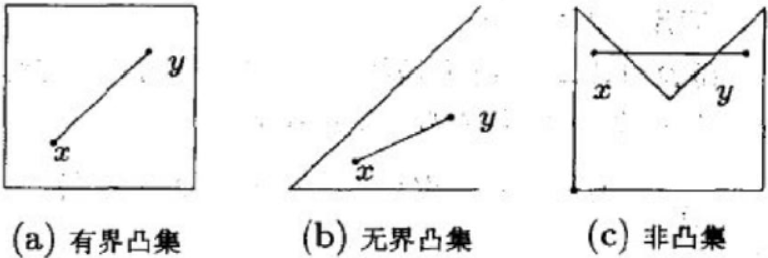
\includegraphics[scale=0.6]{convex_collection.png}
							\renewcommand{\figurename}{Fig} % set picture title starting with Fig or 图
							\caption{convex collection}
							\label{fig:1}
						\end{figure}
				\end{enumerate}
			
		\section{\quad affine transformation}
			\subsection{\quad concept}
				函数 $f(x) = Ax + b$ 的形式, 称函数是放射的: 即线性函数加常数的形式
				
			\subsection{\quad theory}
				\begin{enumerate}
					\item 仿射变换 $f(x) = Ax + b$, $A \in \boldsymbol{\text{R}}^{m \times n}$, $b \in \boldsymbol{\text{R}}^m$
						\begin{enumerate}
							\item 伸缩、平移、投影
						\end{enumerate}
					
					\item 若 $f$ 是仿射变换, $f : \boldsymbol{\text{R}}^n \rightarrow \boldsymbol{\text{R}}^m \ \quad f(S) = \{ f(x) | x \in S \}$
						\begin{enumerate}
							\item 若 $S$ 为凸集, 则 $f(x)$ 为凸集;
							
							\item 若 $f(S)$ 为凸集, 则 $S$ 为凸集. 
						\end{enumerate}
					
					\item 两个凸集的和为凸集
						\begin{align}
							S_1 + S_2 = \{ x + y | x \in S_1, y \in S_2 \}
						\end{align}
						
					\item 两个凸集的笛卡尔积 (直积) 为凸集
						\begin{align}
							S_1 \times S_2 = \{ (x_1, x_2) | x \in S_1, x_2 \in S_2 \}
						\end{align}
						
					\item 两个集合的部分和为凸集 (分配率)
						\begin{align}
							S = \{ (x, y_1 + y_2) | (x, y_1) \in S_1, (x, y_2) \in S_2 \}
						\end{align}
				\end{enumerate}
			
		\section{\quad perspective collineation}
			\subsection{\quad concept}
				透视函数对向量进行伸缩 (规范化), 使得最后一维的分量为 1 并舍弃之.
					\begin{align}
						P : \boldsymbol{\text{R}}^{n+1} \rightarrow \boldsymbol{\text{R}}^{n}, \ P(z, t) = z/t
					\end{align}
			
			\subsection{\quad direct significance}
				小孔成像
				\begin{figure}[H]
					\vspace{-0.2cm}  %调整图片与上文的垂直距离
					\setlength{\abovecaptionskip}{-0.2cm}   %调整图片标题与图距离
					%\setlength{\belowcaptionskip}{-1cm}   %调整图片标题与下文距离
					\centering
					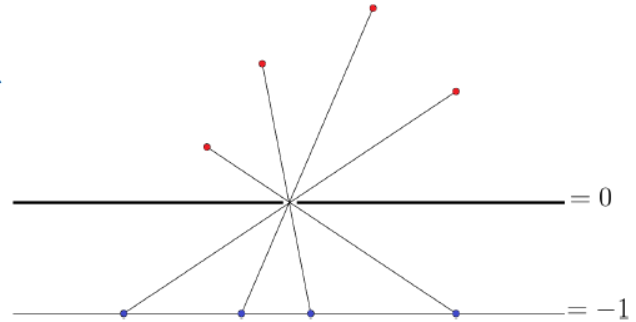
\includegraphics[scale=0.6]{perspective_collineation.png}
					\renewcommand{\figurename}{Fig} % set picture title starting with Fig or 图
					\caption{significance of perspective collineation}
					\label{fig:2}
				\end{figure}
			
			\subsection{\quad summary}
				凸集的透视变换仍然是凸集
				
		\section{\quad segmentation plane}
			\subsection{\quad concept}
				设 C 和 D 为两不相交的凸集, 则存在超平面 P, P可以将 C 和 D 分离.
				\begin{align}
					\forall x \in C, a^T x \leq b \ \text{且} \ \forall x \in D, a^T x \geq b
				\end{align}
				
			\subsection{\quad segmentation plane}
				\begin{figure}[H]
					\vspace{-0.2cm}  %调整图片与上文的垂直距离
					\setlength{\abovecaptionskip}{-0.2cm}   %调整图片标题与图距离
					%\setlength{\belowcaptionskip}{-1cm}   %调整图片标题与下文距离
					\centering
					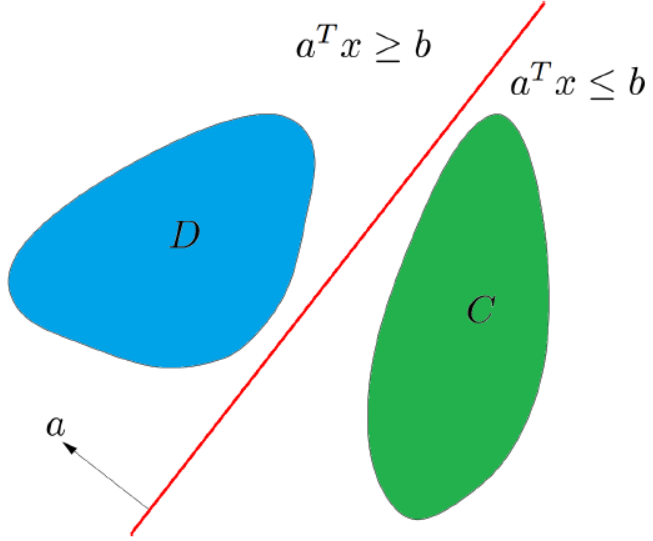
\includegraphics[scale=0.6]{segmentation_plane.png}
					\renewcommand{\figurename}{Fig} % set picture title starting with Fig or 图
					\caption{segmentation plane}
					\label{fig:3}
				\end{figure}
			
			\subsection{\quad the structure of sefmentation plane}
				\begin{enumerate}
					\item 两个集合的距离, 定义为两个集合间元素的最短距离
					
					\item 做集合 C 和集合 D 最短线段的垂直平分线
					
					\item picture
						\begin{figure}[H]
							\vspace{-0.2cm}  %调整图片与上文的垂直距离
							\setlength{\abovecaptionskip}{-0.2cm}   %调整图片标题与图距离
							%\setlength{\belowcaptionskip}{-1cm}   %调整图片标题与下文距离
							\centering
							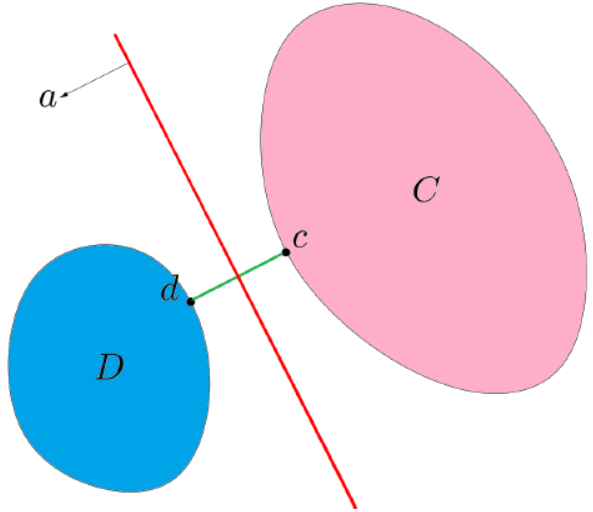
\includegraphics[scale=0.5]{the_distance_of_segmentation.png}
							\renewcommand{\figurename}{Fig} % set picture title starting with Fig or 图
							\caption{the distance of segmentation plane}
							\label{fig:4}
						\end{figure}
				\end{enumerate}
			
			\subsection{\quad support hyperplane}
				\begin{figure}[H]
					\vspace{-0.2cm}  %调整图片与上文的垂直距离
					\setlength{\abovecaptionskip}{-0.2cm}   %调整图片标题与图距离
					%\setlength{\belowcaptionskip}{-1cm}   %调整图片标题与下文距离
					\centering
					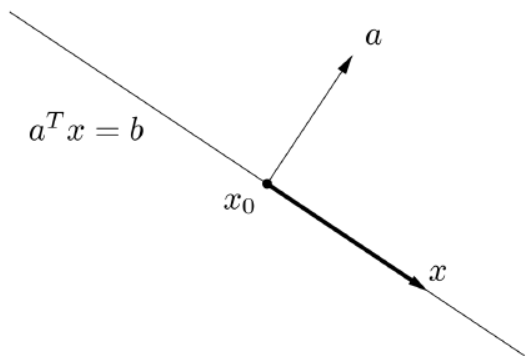
\includegraphics[scale=0.5]{hyperplane.png}
					\renewcommand{\figurename}{Fig} % set picture title starting with Fig or 图
					\caption{hyperplane}
					\label{fig:5}
				\end{figure}
			
				\begin{enumerate}
					\item 设集合 C , $x_0$ 为 C 边界上的点. 若存在 $a \neq 0$, 满足对任意 $x \in C$, 都有 $a^T x \leq a^T x_0$ 成立, 则称超平面 $\{ x | a^T x = a^T x_0 \}$ 为集合 C 在点 $x_0$ 处的支撑超平面.
					
					\item 凸集边界上任意一点, 均存在支撑超平面
					
					\item 反之, 若在一个闭的非中空 (内部点不为空) 集合, 在边界上的任意一点存在支撑超平面, 则该集合为凸集
				\end{enumerate}
			
			\subsection{\quad question}
				\begin{enumerate}
					\item 如何定义两个集合的 “最优” 分割超平面?
						\begin{enumerate}
							\item 找到集合 “边界” 上的若干点, 以这些点为 “基础” 计算超平面的方向; 以两个集合边界上的这些点的平均作为超平面的 “截距”
							
							\item 支持向量: support vector
							
							\item optimal segmentation plane
								\begin{figure}[H]
									\vspace{-0.2cm}  %调整图片与上文的垂直距离
									\setlength{\abovecaptionskip}{-0.2cm}   %调整图片标题与图距离
									%\setlength{\belowcaptionskip}{-1cm}   %调整图片标题与下文距离
									\centering
									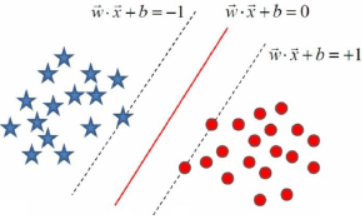
\includegraphics[scale=0.6]{optimal_segmentation_plane.png}
									\renewcommand{\figurename}{Fig} % set picture title starting with Fig or 图
									\caption{optimal segmentation plane}
									\label{fig:6}
								\end{figure}
						\end{enumerate}
					
					\item 若两个集合有部分相交, 如何定义超平面, 使得两个集合 “尽量” 分开?
						\begin{enumerate}
							\item 注: 上述 “集合” 不一定是凸集, 可能是由若干离散点组成. 若一组集合为 $(x, 1)$, 另一组集合为 $(x, 2)$, 则为机器学习中的分类问题.
						\end{enumerate}
				\end{enumerate}
			
		\section{\quad property of convex function}
			\subsection{\quad concept}
				若函数 $fx(x)$ 的定义域 domf 为凸集, 且满足
				\begin{align}
					\forall x, y \in \text{dom} \ f, \ 0 \leq \theta \leq 1, \ \text{有}\\
					f(\theta x + (1-\theta)y) \leq \theta f(x) + (1-\theta)f(y)
				\end{align}
				\begin{figure}[H]
					\vspace{-0.6cm}  %调整图片与上文的垂直距离
					\setlength{\abovecaptionskip}{-0.2cm}   %调整图片标题与图距离
					%\setlength{\belowcaptionskip}{-1cm}   %调整图片标题与下文距离
					\centering
					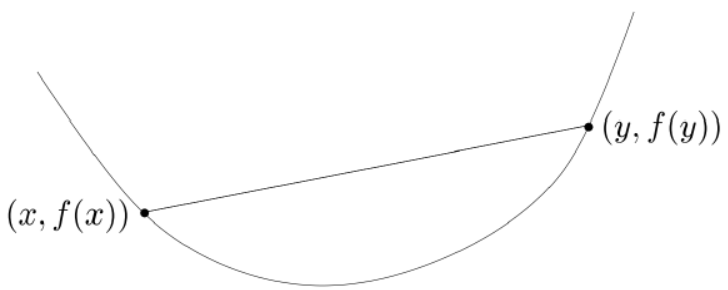
\includegraphics[scale=0.6]{convex_function.png}
					\renewcommand{\figurename}{Fig} % set picture title starting with Fig or 图
					\caption{convex function}
					\label{fig:7}
				\end{figure}
					
			\subsection{\quad first-order derivative of convex function}
				若 $f(x)$ 一阶可微, 则函数 f 为凸函数当前仅当 f 的定义域 domf 为凸集, 且
				\begin{align}
					\forall x, y \in \text{dom} \ f, \ f(y) \geq f(x) + \nabla f(x)^T (y-x)
				\end{align}
				\begin{figure}[H]
					\vspace{-0.6cm}  %调整图片与上文的垂直距离
					\setlength{\abovecaptionskip}{-0.2cm}   %调整图片标题与图距离
					%\setlength{\belowcaptionskip}{-1cm}   %调整图片标题与下文距离
					\centering
					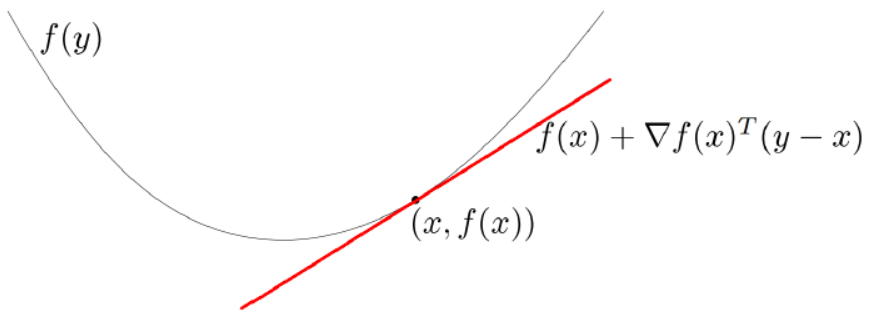
\includegraphics[scale=0.6]{first_derivation_of_convex_function.png}
					\renewcommand{\figurename}{Fig} % set picture title starting with Fig or 图
					\caption{first-order derivative of convex function}
					\label{fig:8}
				\end{figure}
				
				对于凸函数, 其一阶 Taylor 近似本质上是该函数的全局下估计
				
			\subsection{\quad second-order derivative of convex function}
				\begin{enumerate}
					\item 若函数 f 二阶可微, 则函数 f 为凸函数当前仅当 dom 为凸集, 且
						\begin{equation}
							\nabla^2 f(x) \succ = 0
						\end{equation}
						
					\item 若 f 是一元函数, 上式表示二阶导大于等于0
					
					\item 若 f 是多元函数, 上式表示二阶导 Hessian 矩阵半正定
				\end{enumerate}

		\section{\quad examples of convex function}
			\begin{itemize}
				\item 指数函数 $f(x) = e^{ax}$
				
				\item 幂函数 $f(x) = x^a, x \in R^+, a \geq 1 \ \text{或} \ a \leq 0$
				
				\item 负对数函数 $f(x) = -\ln x$
				
				\item 负熵函数 $f(x) = x\ln x$
				
				\item 范数函数 $f(\vec{x}) = \parallel x \parallel$
				
				\item 最大值函数 $f(\vec{x}) = \max (x_1, x_2, ..., x_n)$
				
				\item 指数线性函数 $f(\vec{x}) = \log \left( e^{x_1} + e^{x_2} + ... + e^{x_n} \right)$
			\end{itemize}
			
	\chapter{\quad Convex Optimization}
		\thispagestyle{fancy}
		\section{\quad optimization problem}
			\begin{enumerate}
				\item common format
					\begin{align}
						\begin{split}
						\text{minimize} \ &f_0(x), x \in \boldsymbol{\text{R}}^n \\
						\text{subject to} \ &g_i(x) \leq 0, \ i=1, ..., m \\
						&h_j(x) = 0, \ j=1, ..., p\\
						\text{优化变量} \quad &x \in \boldsymbol{R}^n \\
						\text{不等式约束} \quad &g_i(x) \leq 0\\
						\text{等式约束} \quad &h_j(x) = 0\\
						\text{无约束优化} \quad &m = p = 0	\label{eq:optimization_problem}									
						\end{split}
					\end{align}
					
				\item domain of optimal problem
					\begin{align}
						D = \bigcap\limits_{i=0}^{m} \text{dom} g_i \cap \bigcup\limits_{j=1}^{p} \text{dom} h_j
					\end{align}
					
				\item feasible dot (solution)
					\begin{itemize}
						\item $x \in D$, 满足式 \ref{eq:optimization_problem} 中约束条件
					\end{itemize}
				
				\item feasible domain (feasible collection)
					\begin{itemize}
						\item 所有可行点的集合 
					\end{itemize}
				
				\item optimization value
					\begin{align}
						p^* = \inf \{ f_0(x) | g_i(x) \leq 0, i=1,...,m, h_j(x)=0,j=1,...,p\}
					\end{align}
					
				\item optimization solution
					\begin{align}
						p^* = f_0(x^*)
					\end{align}
			\end{enumerate}
		
		\section{\quad convex optimization}
			\subsection{\quad basic form}
				\begin{align}
					\begin{split}
						\text{minimize} \quad &f_0(x), x \in \boldsymbol{\text{R}}^n \\
						\text{subject to} \quad &g_i(x) \leq 0, i=1,...,m \\
						&h_j(x) = 0, j=1,...,p
					\end{split}
				\end{align}
				\begin{enumerate}
					\item among, $g_i(x)$ 为凸函数, $h_j(x)$ 为仿射函数
					
					\item important property of convex optimization problem
						\begin{enumerate}
							\item 凸优化问题的可行域为凸集
							
							\item 凸优化问题的局部最优解即为 \textcolor{red}{全局最优解}
						\end{enumerate}
				\end{enumerate}
			
			\subsection{\quad Lagrange乘子法}
				在支持向量机模型 (SVM) 的推导中一步很关键的就是利用 Lagrange 对偶性 将原问题转化为对偶问题.
				\begin{enumerate}
					\item theoty: \\
						一般的求极值问题, 求导等于0. 但是如果不但要求极值, 还要求一个满足一定约束条件的极值, 那么此时就可以构造 Lagrange 函数, 其实就是 \textcolor{red}{把约束项添加到原函数上, 然后对构造的新函数求导}
						
					\item example picture
						\begin{figure}[H]
							\vspace{-0.6cm}  %调整图片与上文的垂直距离
							\setlength{\abovecaptionskip}{-0.2cm}   %调整图片标题与图距离
							%\setlength{\belowcaptionskip}{-1cm}   %调整图片标题与下文距离
							\centering
							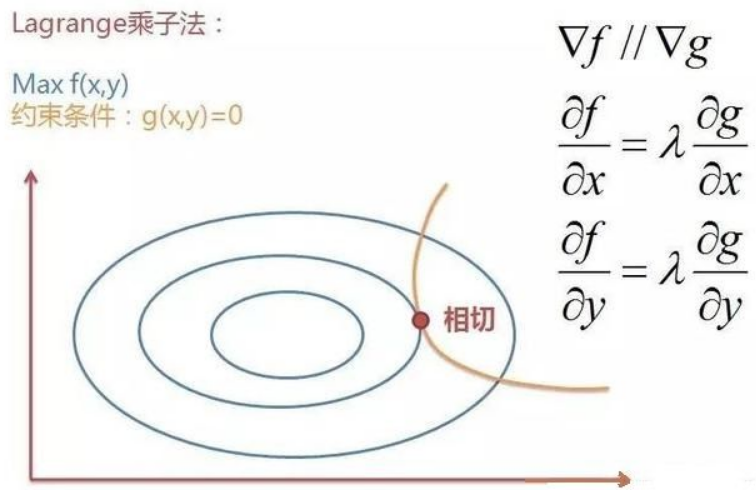
\includegraphics[scale=0.6]{Lagrange_multiplier.png}
							\renewcommand{\figurename}{Fig} % set picture title starting with Fig or 图
							\caption{Lagrange multiplier method}
							\label{fig:9}
						\end{figure}
					
					\item analysis: \\
					对于一个要求极值的函数 $f(x, y)$, 图上的蓝圈就是这个函数的等高图, 就是说 $f(x, y) = c_1, c_2, ..., c_n$ 分别代表不同的数值 (每个值代表一圈, 等高图), 我要找到一组 $(x, y)$, 使它的 $c_i$ 值越大越好, 但是这点必须满足约束条件 $g(x, y)$ (在黄线上)
					
					\item conclusion: \\
					就是说 $f(x, y)$ 和 $g(x, y)$ 相切, 或者说它们的梯度 $\nabla f$ 和 $\nabla g$ 平行, 因此它们的梯度 (偏导) 成倍关系; 那我们就假设为 $\lambda$ 倍, 然后把约束条件加到原函数后再对它求导, 其实就等于满足了图上的式子了.
				\end{enumerate}

					
			
			\subsection{ Lagrange 函数的极小极大最优值 $\min\limits_x\max\limits_{\lambda, \nu: \lambda_i \geq 0} L(x, \lambda, \nu)$ 和 原问题的最优值 $p^*$}
				\begin{enumerate}
					\item 一般优化问题的 Lagrange 乘子法
						\begin{align}
							\begin{split}
								\text{minimize} \quad &f_0(x), x \in \boldsymbol{\text{R}}^n \\
								\text{subject to} \quad &g_i(x) \leq 0, i=1,...,m \\
								&h_j(x) = 0, j=1,...,p
							\end{split}
						\end{align}
						
					\item Lagrange 函数
						\begin{align}
							L(x, \lambda, \nu) = f_0(x) + \sum_{i=1}^{m} \lambda_i g_i(x) + \sum_{j=1}^{p} \nu_j h_j(x) \label{eq2: Lagrange_funtion}
						\end{align}
						对固定的 x, Lagrange 函数 $L(x, \lambda, \nu)$ 为关于 $\lambda$ 和 $\nu$ 的仿射函数, 这里, $x = (x^1, x^2, ..., x^n)^T \in \boldsymbol{\text{R}}^n, \lambda, \nu$ 是	Lagrange 乘子, $\lambda \geq 0$
						
					\item \textcolor{red}{Lagrange 函数的极小极大最优值 $\min\limits_x\max\limits_{\lambda, \nu: \lambda_i \geq 0} L(x, \lambda, \nu)$ 和 原问题的最优值 $p^*$ 之间的关系}
					
					考虑 x 的函数: 
						\begin{align}
							f(x) = \max\limits_{\lambda, \nu : \lambda \geq 0} L (x, \lambda, \nu) \label{eq3: Lagrange and original problem}
						\end{align}
					即\textcolor{red}{原问题 $f(x)$ 与 Lagrange 函数在 乘子变量最大化 时的值是等价的}
					
					\item 证明上式:
					假设给定某个 x, 如果 x 违反原始问题的约束条件, 即存在某个 $i$ 使得 $g_i(x) > 0$ 或者存在某个 $j$ 使得 $h_j(x) \neq 0$, 那么就有
						\begin{align}
							\phi_P(x) = \max\limits_{\lambda, \nu : \lambda \geq 0} \left[ f(x) + \sum_{i=1}^{m} \lambda_i g_i(x) + \sum_{i=1}^{p} \nu_i h_i(x) \right] = +\infty
						\end{align}
					这里, 下标 P 表示原始问题
					
					\item 因为若某个 $i$ 使约束 $g_i(x) > 0$, 则可令 $\lambda_i \rightarrow +\infty$, 若某个 $j$ 使 $h_j(x) \neq 0$, 则可令 $\nu_i$ 使 $\nu_j h_j(x) \rightarrow +\infty$, 而将其余各 $\lambda_i, \nu_j$ 均取为0
					
						\textcolor{red}{如果 $x$ 满足约束条件, 则由式 \ref{eq2: Lagrange_funtion} 和式 \ref{eq3: Lagrange and original problem} 可知, $\phi_P (x) = f(x)$}
					
					\item summary:
						\begin{align}
							\phi_P(x) = \left\{ 
								\begin{matrix}
									&f(x),     &x \ \text{满足原始问题约束} \\
									&+\infty,  &\text{其他}
								\end{matrix}
								\right.
						\end{align}
						所以如果考虑极小化问题
							\begin{align}
								\min\limits_x \phi_P(x) = \min\limits_x \max\limits_{\lambda, \nu : \lambda \geq 0} L(x, \lambda, \nu)
							\end{align}
						\textcolor{red}{它是与原始最优化问题 \ref{eq:optimization_problem} 等价的}, 即它们有相同的解
						
						\textcolor{red}{此时将原始最优化问题表示为广义 Lagrange 函数的极小极大问题.}
						
						为了方便, 定义原始问题的最优值
							\begin{align}
								p^* = \min\limits_x \phi_P (x) = \min f(x)
							\end{align}
						称为原始问题的值
				\end{enumerate}
			
			\subsection{\quad Lagrange 对偶函数 (dual function)}
				\begin{enumerate}
					\item Lagrange 对偶函数, 注意此处 \textcolor{blue}{下式中x需不需要改成$\widetilde{x}$}
						\begin{align}
							\Gamma (\lambda, \nu) = \inf \limits_{x \in D} L(x, \lambda, \nu) = \inf \limits_{x \in D} (f_0(x) + \sum_{i=1}^{m} \lambda_i g_i(x) + \sum_{i=1}^{p} \nu_i h_i(x))
						\end{align}
					
					\item 若 $\widetilde{x} \in \mathbb{D}$ 为主问题 \ref{eq:optimization_problem} 可行域中的点, 则对任意 $\nu$ 和 $\lambda \succeq 0$ 都有
						\begin{align}
							\sum_{i=1}^{m} \lambda_i g_i(x) + \sum_{i=1}^{n} \nu_j h_j(x) \leq 0
						\end{align}
						进而有
						\begin{align}
							\Gamma (\lambda, \nu) = \inf \limits_{x \in D} L(x, \lambda, \nu) \leq \inf L(\widetilde{x}, \lambda, \nu)
							\leq f(\widetilde{x})
						\end{align} 
					\item 若没有下确界, 定义 \textcolor{red}{主问题下界}:
						\begin{align}
							\Gamma (\lambda, \nu) = -\infty
						\end{align}
						
					\item 根据定义, 显然有: 对 $\forall \lambda > 0, \ \forall \nu$, 若原优化问题有最优值 $p^*$, 则
						\begin{align}
							\Gamma (\lambda, \nu) \leq p^*
						\end{align}
						即对偶函数给出了主问题的最优值的下界, 显然, 这个下界取决于 $\lambda$ 和 $\nu$ 的值. 于是, 一个很自然的问题是: 基于对偶函数能获得的最好下界是什么?
						
					\item 上述引出了 \textcolor{red}{对偶优化问题}
						\begin{align}
							\max \Gamma (\lambda, \nu) \quad \text{s.t.} \ \lambda \succeq 0 \label{eq1:optimal_problem}
						\end{align}
						式 \ref{eq1:optimal_problem} 就是 主问题 \ref{eq:optimization_problem} 的对偶问题, 其中 $\lambda$ 和 $\nu$ 称为 “对偶变量” (dual variable)
						
					\item 进一步: 无论主问题的 \ref{eq:optimization_problem} 的凸性如何, 对偶问题 Lagrange 对偶函数 \ref{eq1:optimal_problem} 始终是凹函数
					
					\item 假设式 \ref{eq1:optimal_problem} 的最优值为 $d^* = \max\limits_{\lambda, \nu} \Gamma(\lambda, \nu)$ , 也即 主问题 \ref{eq:optimization_problem} 中 最优值 $p^*$ 的下界
					
					\item 显然有 $d^* = \max\limits_{\lambda, \nu} \Gamma(\lambda, \nu) \leq p^*$, 这称为 “弱对偶性” (weak duality) 成立; 
					
					  	  若 $d^* = \max\limits_{\lambda, \nu} \Gamma(\lambda, \nu) = p^*$, 则称为 “强对偶性” (strong duality) 成立, 此时由对偶问题能获得主问题的最优下界. 
						
					\item 对于一般优化问题, 强对偶性通常不成立. 但是, 若主问题为凸优化问题, 如式 \ref{eq:optimization_problem} 中 $f(x)$ 和 $g_j(x)$ 均为凸函数, $h_i(x)$ 为仿射函数, 且其可行域中至少有一点使不等式约束严格成立, 此时强对偶性成立. 注意: 在强对偶性成立时, 将 Lagrange 函数对原变量求导, 并令导数等于0, 即可得到 原变量 与 对偶变量的数值关系. 
					
					\item 上述分析, 若满足强对偶性的 KKT 条件, 此时: 
						\begin{align}
							\begin{split}
								d^* &= \max\limits_{\lambda, \nu: \lambda_i \geq 0} \min\limits_x L(x, \lambda, \nu) = \min\limits_x\max\limits_{\lambda, \nu: \lambda_i \geq 0} L(x, \lambda, \nu) \\
								&= p^* = \min f(x) \quad \{ x \ \text{subject to 约束条件} \}
							\end{split}
						\end{align}
					 
					 \item prove:\\ 若原始问题和对偶问题都有最优值, 则 $d^* = \max\limits_{\lambda, \nu: \lambda_i \geq 0} \min\limits_x L(x, \lambda, \nu) \leq \min\limits_x\max\limits_{\lambda, \nu: \lambda_i \geq 0} L(x, \lambda, \nu) 
					 = p^* = \min f(x) \quad \{ x \ \text{subject to 约束条件} \}$
					 
					 process:\\
						 对任意的 $\lambda, \nu$ 和 $x$, 有
						 	\begin{align}
					 			L(x, \lambda, \nu) \leq \max\limits_{\lambda, \nu : \lambda \geq 0} L(x, \lambda, \nu)
					 		\end{align}
					 		\begin{align}
					 			\therefore \quad  \Gamma_D (\lambda, \nu) = \min\limits_x L(x, \lambda, \nu) \leq L(x, \lambda, \nu) \leq \max\limits_{\lambda, \nu : \lambda \geq 0} L(x, \lambda, \nu) = \phi_P (x)
					 		\end{align}
					 `	即: 
					 		\begin{align}
					 			\Gamma_D (\lambda, \nu) \leq \phi_P (x)
					 		\end{align}
					 	由于原始问题和对偶问题均有最优值
					 		\begin{align}
					 			\therefore \quad \max\limits_{\lambda, \nu : \lambda \geq 0} \Gamma_D (\lambda, \nu) \leq \min\limits_x \phi_P (x)
					 		\end{align}
					 	即:
					 		\begin{align}
					 			\begin{split}
					 				d^* &= \max\limits_{\lambda, \nu: \lambda_i \geq 0} \min\limits_x L(x, \lambda, \nu) \leq 	\min\limits_x\max\limits_{\lambda, \nu: \lambda_i \geq 0} L(x, \lambda, \nu) \\
					 				&= p^* = \min f(x) \quad \{ x \ \text{subject to 约束条件} \}
					 			\end{split}
					 		\end{align}
					 						 	
					 \item KKT 条件:
					 	\begin{align}
					 		g_i(x^*) &\leq 0, \quad i=1,2,..,k 
					 		\\
					 		\lambda_i^* &\geq 0, \quad i=1,2,...,k 
					 		\\
					 		\begin{split}
					 			\lambda_i^* g_i(x^*) &= 0, \quad i=1,2,...,k
					 		\end{split} \label{eq6: dual complementary condition}
					 		 \\
					 		h_j(x^*) &= 0, \quad j=1,2,...,l 
					 		\\
					 		\begin{split}
					 			\nabla L(x^*, \lambda^*, \nu^*) &= \nabla f(x^*) + \sum_{i=1}^{k} \lambda_i^* \nabla g_i(x^*) + \sum_{j=1}^{l} \nu_i^* \nabla h_j (x^*) = 0 
					 		\end{split} \label{eq5: all variable derivation of Lagrange function}
					 	\end{align}
					 	上式中 \ref{eq5: all variable derivation of Lagrange function} 等价于
					 	\begin{align}
					 		\left\{
					 			\begin{matrix}
					 				\nabla_x L(x^*, \lambda^*, \nu^*) = 0 \\
					 				\nabla_\lambda L(x^*, \lambda^*, \nu^*) = 0 \\
					 				\nabla_\nu L(x^*, \lambda^*, \nu^*) = 0
					 			\end{matrix}
					 		\right.
					 	\end{align}
					 	
					 	特别指出, 式 \ref{eq6: dual complementary condition} 称为 KKT 的对偶互补条件. 由此条件可知: 若 $\lambda_i^* > 0$, 则 $g_i(x^*) = 0$
					 	
					 	上式中, $x^*$ 是原始变量的解, $\lambda^*, \nu^*$ 是对偶变量的解, 并且 $p^* = d^* = L(x^*, \lambda^*, \nu^*)$
					 	
					\item 左侧是原函数, 右侧为对偶函数
						\begin{figure}[H]
							\vspace{-0.3cm}  %调整图片与上文的垂直距离
							\setlength{\abovecaptionskip}{-0.05cm}   %调整图片标题与图距离
							%\setlength{\belowcaptionskip}{-1cm}   %调整图片标题与下文距离
							\centering
							\subfigure[Original function]{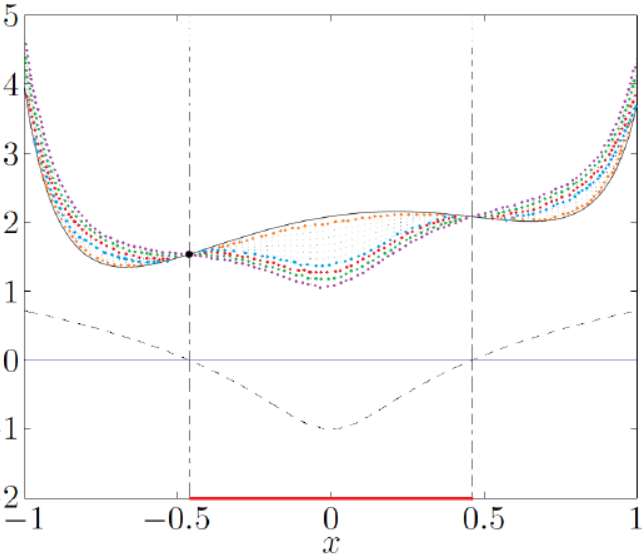
\includegraphics[height=5cm,width=6cm]{original_function_dual_problem.png}}
							%scale=0.6, height=4cm,width=4cm
							\qquad
							\subfigure[Dual function]{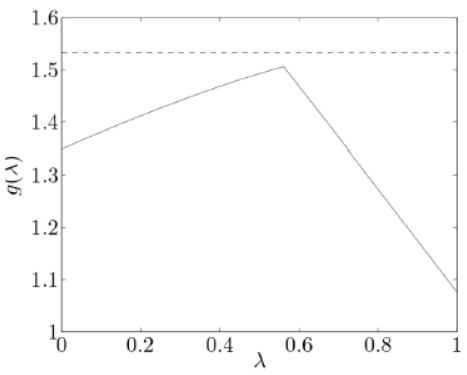
\includegraphics[height=5cm,width=6cm]{dual_function_dual_problem.png}}
							\renewcommand{\figurename}{Fig} % set picture title starting with Fig or 图
							\caption{ dual problem }
							\label{fig:9}
						\end{figure}
					
					
					SVM 里的 w,b 看做是 Lagrange 函数里的变量 x 
				\end{enumerate}
				
	\chapter{\quad SVM}
		\section{\quad jiange}
	
\end{document}